% WACV 2027 submission, Evaluations and Datasets track.
\documentclass[10pt,twocolumn,letterpaper]{article}

\usepackage[review,datasets]{wacv}

\input{preamble}

\definecolor{wacvblue}{rgb}{0.21,0.49,0.74}
\usepackage[pagebackref,breaklinks,colorlinks,allcolors=wacvblue]{hyperref}

\usepackage{graphicx}
\usepackage{amsmath}
\usepackage{amssymb}
\usepackage{booktabs}
\usepackage{multirow}
% cleveref is already loaded by wacv.sty (line 519) with [capitalize];
% loading it again causes an option clash.
\usepackage{amsthm}
\newtheorem{proposition}{Proposition}
\newtheorem{corollary}{Corollary}
% wacv.sty loads cleveref at \AtEndPreamble and sets the house style there:
% \cref gives "Sec." and \Cref gives "Section". We use \Cref for sections
% throughout and \cref for equations, tables and figures.

\def\wacvPaperID{*****} % *** Enter the WACV Paper ID here
\def\confName{WACV}
\def\confYear{2027}

\newcommand{\kap}{\kappa}
\newcommand{\A}{\mathcal{A}}
% \mathbb{1} is not a glyph in the default fonts and renders as a struck symbol.
\newcommand{\ind}[1]{\mathbf{1}\!\left[ #1 \right]}
\newcommand{\own}{\mathrm{own}}
\newcommand{\oth}{\mathrm{oth}}

\begin{document}

\title{Crop Alignment: A Structural-Null Test for Closed-Loop Labels\\
in Segmentation Benchmarks}

% Keep the release anonymous until the camera-ready author list is known.
\author{Anonymous Authors}

\maketitle

\begin{abstract}
Many segmentation benchmarks are labelled by algorithms, not by people. When the labelling rule reads the same pixels the model reads, the
benchmark closes a loop: a label stops being a property of the ground and becomes a
function of the window it was computed in, and a model can score well by reproducing
the labeller instead of the phenomenon. We give a test for this, calibrate it, and
apply it.

The test asks, on pixels where overlapping crops disagree, how much more often a
model predicts the label of the crop it is currently reading than the label a
different crop assigns the same physical pixel. On any nonempty disagreement set,
we prove this quantity is zero for a predictor whose output does not depend on the
crop. The null is structural, so it carries no sampling error and needs no control
arm to estimate. Run on a per-pixel threshold, which is crop-invariant by
construction, our estimator returns $|\kappa| < 1.4 \times 10^{-15}$. The scope is
deliberately narrow: the test has no support when crops never disagree and cannot
diagnose crop-invariant pseudo-label shortcuts or shortcuts unrelated to crop
geometry.

A structural null shows the test reads zero in a known negative control. It does not
show the test is right when crop dependence is present, so we build a labeller whose
crop dependence we set with a dial. In the released event-level summaries, crop
alignment rises from $+0.0569$ to $+0.2476$ across that dial and is ordered correctly
with it in 10 of 11 held-out events. Over the same sweep, accuracy against expert
labels falls by $0.1056$ mIoU ($t=-4.27$), and $\kappa$ tracks that loss at fixed dial
settings.

On a published sea-ice benchmark whose labeller we recover exactly, the 16 folds
with committed machine-readable evidence give crop alignment $+0.1230$ for the
benchmark labels and $+0.0157$ for a matched control: a paired difference of
$+0.1073$ ($t=12.88$, positive in all 16 folds). We release the test as a single
file; it reproduces the committed aggregate to floating-point precision. The
release does not contain the raw predictions or checkpoints needed to reproduce
training end to end, and we state that evidence boundary explicitly.
\end{abstract}

\section{Introduction}
\label{sec:intro}

Auto-labelling made large segmentation benchmarks possible. It also made some of
them circular, because the label is a deterministic function of the image the model
receives. One measurable form of that circularity occurs when the labeller is run on
crops and its answer changes with the crop. That failure is widely acknowledged and
rarely quantified, in part because there has been no estimand with a value known in
advance under the null that can be computed on a benchmark you did not build.

This paper supplies one. We define crop alignment, prove its null, calibrate it
against a labeller we control, measure what the thing it detects costs against human
annotation, and release an implementation that runs on other people's data. We apply
it to two benchmarks, and \Cref{sec:wild,sec:resolution} report what it finds there.

Foundation-model masks are increasingly used as ground
truth~\cite{kirillov2023segment}. When those masks are generated crop by crop, they
can inherit the property tested here; scene-level pseudo-labels can still close the
input--label loop but fall outside our diagnostic if they are crop-invariant. The
adjacent literatures in \Cref{sec:related} diagnose related failures after the fact.
What is scarce is a controlled measurement of this crop-dependent case.

\paragraph{Terms.} A benchmark is \emph{closed-loop} when its labels are computed
from the model's own input. \emph{Crop alignment} ($\kap$) is defined in
\Cref{sec:kappa} and audits only the crop-dependent subset of such benchmarks. The
\emph{artefact premium} is defined in
\Cref{sec:resolution}, where it is also estimated.

\section{Related work}
\label{sec:related}

Closed-loop labelling sits between five literatures. The distinction this paper
turns on is the one between shortcut learning and label noise.

\paragraph{Shortcut learning.} Documented cases include
hospital-specific tokens in chest radiographs~\cite{zech2018variable}, background
rather than animal in wildlife recognition~\cite{beery2018terra}, and the general
account of shortcut learning as a property of gradient descent rather than of any
one dataset~\cite{geirhos2020shortcut, lapuschkin2019unmasking}. In each case the cue was identified after a model had already been trained and seen
to generalise badly. Crop alignment is a forward test with a value known under the
null, so it can be run before anyone has been surprised, and it names the cue in
advance.

\paragraph{Annotation artefacts.} The closest analogue is not in vision.
Hypothesis-only baselines on natural language inference showed that labels were
partly predictable from properties of the annotation process, and that leaderboard
progress had been measuring that predictability~\cite{gururangan2018annotation,
poliak2018hypothesis}. The failure is the same. The difference is that a
crowdworker's habits cannot be recovered, whereas an algorithmic labeller can be. We
invert one labeller to its constant in 17 of 17 folds and recover another labeller's
threshold and its preprocessing kernel to within 0.25\,dB on 10 of 10
events. Exact recovery lets us build the artefact with a dial instead of only detecting
it.

\paragraph{Label noise, and why this is not that.} The standard frame for imperfect
labels is noise, with a large literature on robust losses, noise-transition
estimation, and the observation that many test labels in standard benchmarks are
simply wrong~\cite{song2022learning, northcutt2021confident,
northcutt2021pervasive}. Closed-loop labels are the opposite of noise. Noise is
unpredictable from the input, so a model cannot learn it. A crop-dependent label is
deterministic in the model's own input, so a model learns it exactly. That is why
closed-loop labels inflate measured performance where noise depresses it. Treating closed-loop labels as noise
prescribes the wrong remedy, because robustness to them makes a model worse on the
benchmark and better on the truth.

\paragraph{Weak and programmatic supervision.} Labelling functions and
foundation-model pseudo-labels are the practice that produces closed-loop labels at
scale~\cite{ratner2017snorkel}. We measure one failure mode of that practice, and
the failure is about where the labelling function reads from. A rule applied once per scene is
fine. The same rule applied per crop is not.

\paragraph{Benchmark statistics.} A separate line argues that benchmark comparisons
are routinely reported without the variance or the power to support them, that seed
and data-order variation can exceed the differences being
claimed~\cite{bouthillier2021accounting, reimers2017reporting}, and that many
published effects are underpowered~\cite{card2020little, damour2022underspecification}.
Our required-sample-size framing in \Cref{sec:resolution} applies that argument to
a benchmark whose independent unit is the acquisition and not the patch, and follows
the standard practice of fixing a margin in advance~\cite{lakens2017equivalence}.

\paragraph{Spatial validation.} In remote sensing and ecology, splitting
spatially autocorrelated data at random inflates measured
skill~\cite{roberts2017cross, ploton2020spatial}, and treating correlated
observations as independent replicates has a name and a long
history~\cite{hurlbert1984pseudoreplication}. Our protocol repairs are the standard
remedies applied to a benchmark that used none of them. What we add is not the
remedies but a measurement of what skipping them costs, stated as a required sample
size.

\section{Crop alignment}
\label{sec:kappa}

\subsection{Definition}

A labeller produces, for each crop $c$ and each pixel $p$ inside it, a label
$L_c(p)$. When it reads only the pixels inside the crop, two crops covering the same
source pixel can assign it different labels. A predictor $f$ maps a pixel and the
crop it is read in to a class, written $f(p \mid c)$.

For a source pixel $p$, let $C(p)$ be the set of crops covering it and
$m(p) = |C(p)|$. The \emph{artefact set} is
\begin{equation}
\A = \{\, p : \exists\, c, c' \in C(p) \text{ with } L_c(p) \neq L_{c'}(p) \,\}.
\label{eq:aset}
\end{equation}
Off $\A$ the labeller is locally single-valued and there is nothing to detect. A
pixel covered by one crop can never enter $\A$, so $m(p) \geq 2$ throughout.

For $p \in \A$ and $c \in C(p)$, with $\ind{\cdot}$ the indicator, define
\begin{align}
\own(p,c) &= \ind{f(p \mid c) = L_c(p)}, \label{eq:own}\\
\oth(p,c) &= \frac{1}{m(p)-1} \sum_{c' \neq c} \ind{f(p \mid c) = L_{c'}(p)},
\label{eq:oth}
\end{align}
where here and below sums over $c$ or $c'$ run over $C(p)$. Then
\begin{equation}
\kap = \mathbb{E}\big[\, \own(p,c) - \oth(p,c) \,\big],
\label{eq:kappa}
\end{equation}
when $\A$ is nonempty, with the expectation taken uniformly over instances $(p,c)$
with $p \in \A$, or under
any weighting that is exchangeable across the crops covering a given pixel.
\Cref{eq:own} asks whether the prediction matches the label of the crop being read.
\Cref{eq:oth} asks how often it matches the label of a different crop covering the
same pixel, averaged so that pixels with more coverage are not overweighted.

\subsection{The null is structural}

\begin{proposition}
\label{prop:null}
Suppose $\A$ is nonempty. Let $f$ be crop-invariant on $\A$, meaning
$f(p \mid c) = f(p)$ for every
$p \in \A$ and every $c \in C(p)$. Then $\kap = 0$ exactly.
\end{proposition}

\begin{proof}
Fix $p \in \A$, write $m = m(p)$ and $y = f(p)$, which by hypothesis does not depend
on the crop. For each class $k$ let $n_k = |\{ c \in C(p) : L_c(p) = k \}|$, so that
$\sum_k n_k = m$. Summing \cref{eq:own} over the crops covering $p$,
\begin{equation}
\sum_{c} \own(p,c) = \sum_{c} \ind{y = L_c(p)} = n_y .
\label{eq:sumown}
\end{equation}
Summing \cref{eq:oth} and exchanging the order of summation,
\begin{align}
\sum_{c} \oth(p,c)
  &= \frac{1}{m-1} \sum_{c} \sum_{c' \neq c} \ind{y = L_{c'}(p)} \nonumber \\
  &= \frac{1}{m-1} \sum_{c'} \ind{y = L_{c'}(p)} \cdot (m-1) \nonumber \\
  &= n_y ,
\label{eq:sumoth}
\end{align}
because each $c'$ is counted once for every $c$ other than itself, that is $m-1$
times, and the normaliser cancels it.

So \cref{eq:sumown} and \cref{eq:sumoth} agree at every $p \in \A$. The average in
\cref{eq:kappa} over all $N$ instances is
\begin{equation}
\kap = \frac{1}{N} \sum_{p \in \A} \ \sum_{c} \big[ \own(p,c) - \oth(p,c) \big] = 0,
\end{equation}
since the inner sum vanishes for each $p$, whatever its coverage.
\end{proof}

Nothing in the argument uses the number of classes, the label distribution, the
coverage $m(p)$, the positive size of $\A$, or any property of the imagery. There is
no sampling error on this null, and no control arm is needed to estimate it. If
$\A$ is empty, however, $\kap$ has no observations and is not defined; emptiness is
not evidence that the labels are free of other shortcuts.

\begin{corollary}
\label{cor:dep}
$\kap \neq 0$ certifies that $f$ is crop-dependent on $\A$.
\end{corollary}

Attributing a positive $\kap$ to a model having learned the \emph{labeller} requires
the matched control of \Cref{sec:floor}, because a network trained on
crop-invariant labels also reads positive.

\subsection{Why the measured control is not zero}
\label{sec:floor}

A convolutional network reading crops is not a crop-invariant predictor. Zero
padding at the crop border, receptive fields truncated at the window edge, and any
normalisation computed over the crop all make $f(p \mid c)$ depend on $c$ near
boundaries. We measure this directly as $\Omega$, the probability that two crops
covering the same pixel yield different predictions. It is $0.032$ for sea-ice
models trained on repaired labels and $0.081$ for flood models at the zero setting
of the dial in \Cref{sec:calib}.

The empirical control therefore sits a little above zero, at $+0.0157$ and
$+0.0569$ respectively. That value is a resolution floor, not a failure of
\cref{prop:null}: the proposition describes a crop-invariant predictor, and a
network is not one. Every result below is the contrast between a closed-loop arm and
its matched control, never raw $\kap$.

\section{Verifying the estimator, and bounding its scope}
\label{sec:verify}

\subsection{A case with a known answer}

\cref{prop:null} supplies something rarer than a null: an input whose correct output
is known before looking, and therefore a test of the code rather than of the data. A
per-pixel threshold on chip-level smoothed VH reads one pixel value and cannot see a
window, so it is crop-invariant literally, not approximately. The estimator
must return zero.

Measured on four held-out flood events, on the same artefact set as every other arm
and between 9.5 and 41 million instances per event, $|\kap|$ is
$6.8 \times 10^{-16}$, $1.3 \times 10^{-15}$, $1.0 \times 10^{-15}$ and
$8.5 \times 10^{-16}$, with $\Omega$ exactly zero in all four. The two probabilities
in \cref{eq:kappa} agree to every printed digit, $0.5977$ against $0.5977$ for the
first event. What remains is accumulated floating-point rounding.

Any error in the $(m-1)$ normaliser, the own-versus-other bookkeeping, or the
artefact-set mask would surface here as a nonzero number. Anywhere else it surfaces
as a plausible
one somewhere it could not be caught.

\subsection{$\kap$ is relative to the crop grid}
\label{sec:grid}

$\kap$ is measured on pixels where covering crops disagree, and how densely crops
are sampled is a choice we made. We tested whether the number survives that choice
by thinning the evaluation grid from stride 32 to stride 64 on identical models and
labels. The sparser grid is a strict subset, so nothing was recomputed and nothing
retrained.

\begin{table}[tb]
\centering
\small
\begin{tabular}{lccc}
\toprule
grid & crops/pixel & artefact set & $\kappa$ contrast \\
\midrule
stride 32 & 16 & 24.71\% & $+0.1907$ \\
stride 64 & 4  & 16.31\% & $+0.3260$ \\
\bottomrule
\end{tabular}
\caption{Crop alignment measured on the same models and labels through two
evaluation grids, the sparser one a strict subset of the denser.}
\label{tab:grid}
\end{table}

It moves, by $1.71\times$ (\cref{tab:grid}). The sparser grid reads a larger
alignment, because the artefact set shrinks to the pixels the crops disagree about
most strongly and the second term of \cref{eq:kappa} averages over fewer and more
distant crops. What survives is the ranking. The two geometries order the eleven
events at $r = +0.984$.

The scope of the instrument is therefore narrower than it first appears. $\kap$
compares arms evaluated on the same crop geometry. Its absolute magnitude is not comparable across papers that tile
differently, and a $\kap$ reported without its crop size and stride cannot be
interpreted. Every comparison in this paper is made within a fixed grid.

\section{Calibrating the test}
\label{sec:calib}

The sea-ice benchmark cannot establish sensitivity, because the crop-dependence of
that pipeline is the unknown being estimated. So we built a labeller with a dial. Sen1Floods11~\cite{bonafilia2020sen1floods11}
ships an Otsu-on-VH~\cite{otsu1979threshold} label set computed once per chip, whose
preprocessing we recover in \Cref{sec:recovery}. Holding that smoothing at the chip
level and recomputing only the threshold inside each crop reproduces the sea-ice
mechanism with one scalar per crop as the entire source of crop-dependence:
\begin{equation}
\tau_c(\alpha) = (1-\alpha)\,\tau_{\text{chip}} + \alpha\,\tau_{\text{crop}} .
\label{eq:dial}
\end{equation}
At $\alpha = 0$ the labels are crop-invariant by construction. At $\alpha = 1$ the
labeller is fully closed-loop. The measured spread of per-crop thresholds within a
chip is 6.13\,dB, so the dial has real range.

The artefact set is fixed at the $\alpha = 1$ labels and every arm is scored on
those same pixels. Without that, the artefact set would shrink as $\alpha$ fell and vanish at
$\alpha = 0$, leaving the control with no pixels to be null on. The sea-ice control
works the same way, evaluating a scene-trained model against the original labels.

\begin{figure}[tb]
\centering
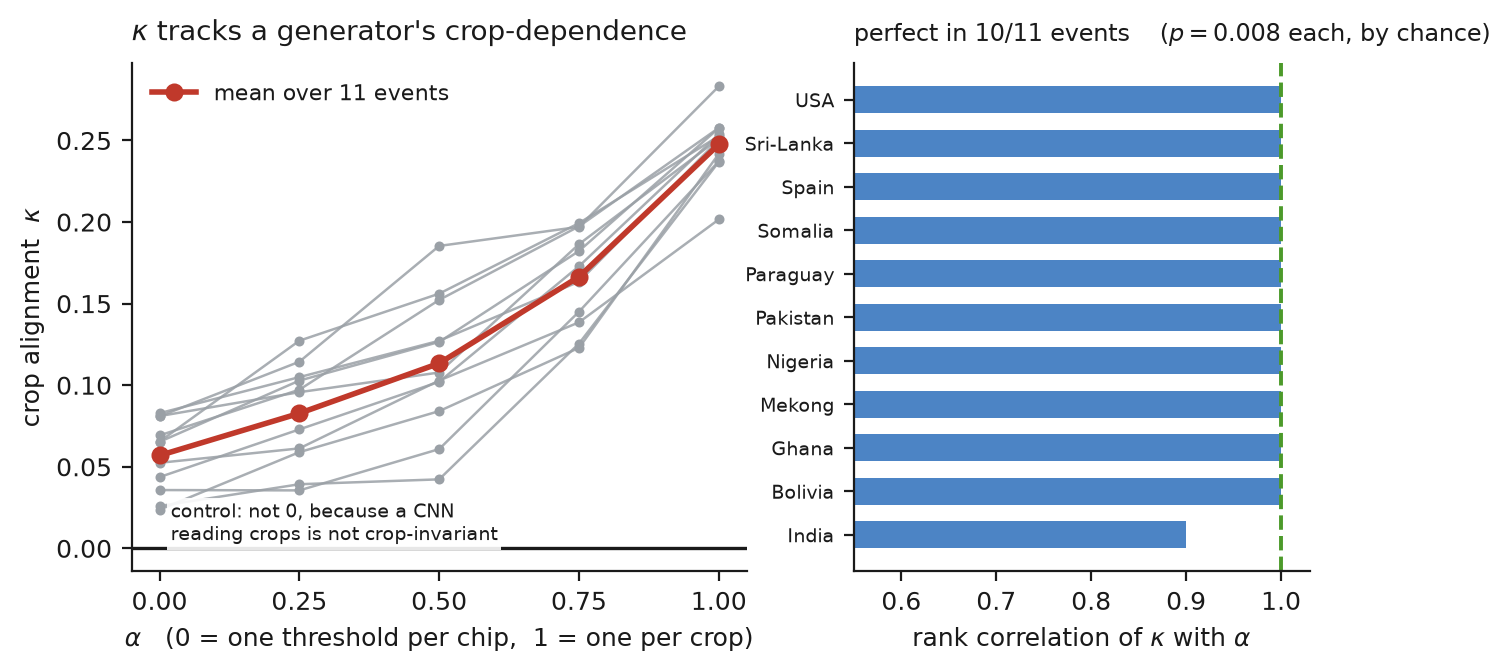
\includegraphics[width=\linewidth]{figures/controlled_calibration.png}
\caption{$\kap$ against the dial of \cref{eq:dial}. Grey lines are held-out events,
red is the mean. Right: rank correlation of $\kap$ with $\alpha$ per event.}
\label{fig:calib}
\end{figure}

\begin{table}[tb]
\centering
\small
\setlength{\tabcolsep}{4pt}
\begin{tabular}{lccccc}
\toprule
$\alpha$ & 0.00 & 0.25 & 0.50 & 0.75 & 1.00 \\
\midrule
$\kap$   & $+0.0569$ & $+0.0828$ & $+0.1134$ & $+0.1664$ & $\mathbf{+0.2476}$ \\
$\Omega$ & 0.0807 & 0.0841 & 0.0897 & 0.0977 & 0.1135 \\
\bottomrule
\end{tabular}
\caption{Crop alignment and model crop-dependence against the dial of
\cref{eq:dial}, averaged over the eleven held-out events.}
\label{tab:calib}
\end{table}

\cref{tab:calib} and \cref{fig:calib} give the result. The contrast between the ends
is $+0.1907$ (sd $0.0212$, $t = 29.84$), positive in 11 of 11 events, sign test
$p = 0.00098$. Per-event rank correlation with $\alpha$ averages $+0.991$ and is
perfect in 10 of 11 events. The exception is a $0.0002$ inversion at the floor
between $\alpha = 0$ and $\alpha = 0.25$.

Positivity on closed-loop labels alone could be accidental. Reproducing the
ordering across five settings, within each event, is harder to get by accident: a
single event ordering five levels correctly by chance has $p = 1/120$.

\paragraph{Scope.} Sen1Floods11 as published computes one threshold per chip, so the
closed-loop artefact is not present in that benchmark. The imagery and the labeller
are real and the crop-dependence is ours. This is a calibration, not a second
sighting in the wild, and nothing here bears on that dataset's published labels.

\section{What closed-loop labels cost}
\label{sec:cost}

\subsection{Against human annotation}

The 55 models from the dial sweep were trained, validated and tested entirely
inside their own labeller, and had never been scored against the expert labels the
dataset ships. Scoring them against the human required no new training.

We score by mosaic: one decision per source pixel, taken by majority vote of the
crops covering it, compared once against the expert label. Patch scoring would count
each pixel about sixteen times and would hand the crop-dependent arms exactly the
reward this paper says patch scoring hands them, which would manufacture the result
rather than measure it.

\begin{figure}[tb]
\centering
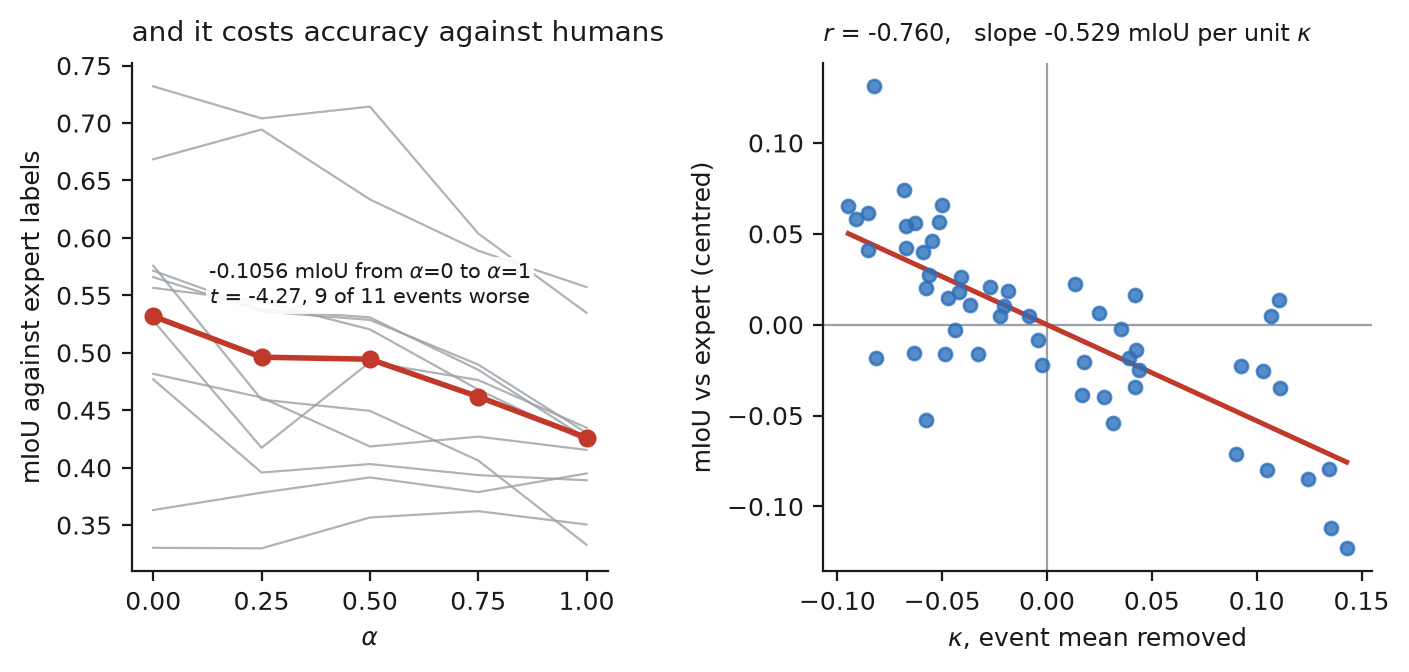
\includegraphics[width=\linewidth]{figures/shortcut_cost.png}
\caption{Left: mIoU against expert labels falls as the labeller becomes more
crop-dependent. Right: $\kap$ against that mIoU with each event's mean removed, so
the slope cannot come from events differing in difficulty.}
\label{fig:cost}
\end{figure}

\begin{table}[tb]
\centering
\small
\setlength{\tabcolsep}{3pt}
\begin{tabular}{lccccc}
\toprule
$\alpha$ & 0.00 & 0.25 & 0.50 & 0.75 & 1.00 \\
\midrule
mIoU vs expert & 0.5318 & 0.4962 & 0.4944 & 0.4618 & $\mathbf{0.4262}$ \\
\bottomrule
\end{tabular}
\caption{Accuracy against expert labels over the dial sweep of \cref{eq:dial},
mosaic scored.}
\label{tab:cost}
\end{table}

Accuracy against the expert labels falls monotonically with the dial
(\cref{tab:cost}). The cost of full crop-dependence is $-0.1056$ mIoU (sd $0.0821$,
$t = -4.27$), worse in 9 of 11 events. Pooled across the sweep with each event's
mean removed, $\kap$ tracks that loss at $r = -0.760$, a slope of $-0.529$ mIoU per
unit $\kap$ ($t = -8.50$), shown in the right panel of \cref{fig:cost}. Two events improve, by $+0.0318$ and $+0.0203$, both among the
lowest-mIoU events in the set. Absolute values are lower than this dataset's
whole-chip numbers because these are $128 \times 128$ crop-trained models with less
context; the quantity in use is the comparison across the dial, not the level.

\subsection{Is $\kap$ only a proxy for the dial?}

The dial moves $\kap$ and the damage together, so a correlation between them is
equally consistent with $\kap$ being a bystander. We therefore hold $\alpha$ fixed
and ask whether $\kap$ still separates events once the dial cannot vary.

\begin{table}[tb]
\centering
\small
\setlength{\tabcolsep}{3pt}
\begin{tabular}{lcccccc}
\toprule
$\alpha$ & 0.00 & 0.25 & 0.50 & 0.75 & 1.00 & mean \\
\midrule
$r$ & $-0.614$ & $-0.698$ & $-0.542$ & $-0.567$ & $-0.534$ & $\mathbf{-0.591}$ \\
\bottomrule
\end{tabular}
\caption{Correlation between $\kap$ and mIoU against expert labels, computed across
the eleven events separately at each dial setting.}
\label{tab:fixed}
\end{table}

All five settings give a negative correlation (\cref{tab:fixed}). Two are
individually significant at $n = 11$, the strongest at $p = 0.017$, and the other
three fall between $p = 0.069$ and $p = 0.091$. The five arms are not independent,
since the dial nests them by construction and they share the same eleven events, so
what the table shows is consistency across the sweep and not five separate tests. At
any fixed level of crop-dependence, the events where the model aligned more with the
crop labeller did worse against the human.

We do not claim $\kap$ is the mechanism by which the damage happens. That would need
a mediation design this experiment does not have. We claim it is an indicator that
survives removing the confound.

\section{Experimental setup}
\label{sec:setup}

\begin{figure*}[t]
\centering
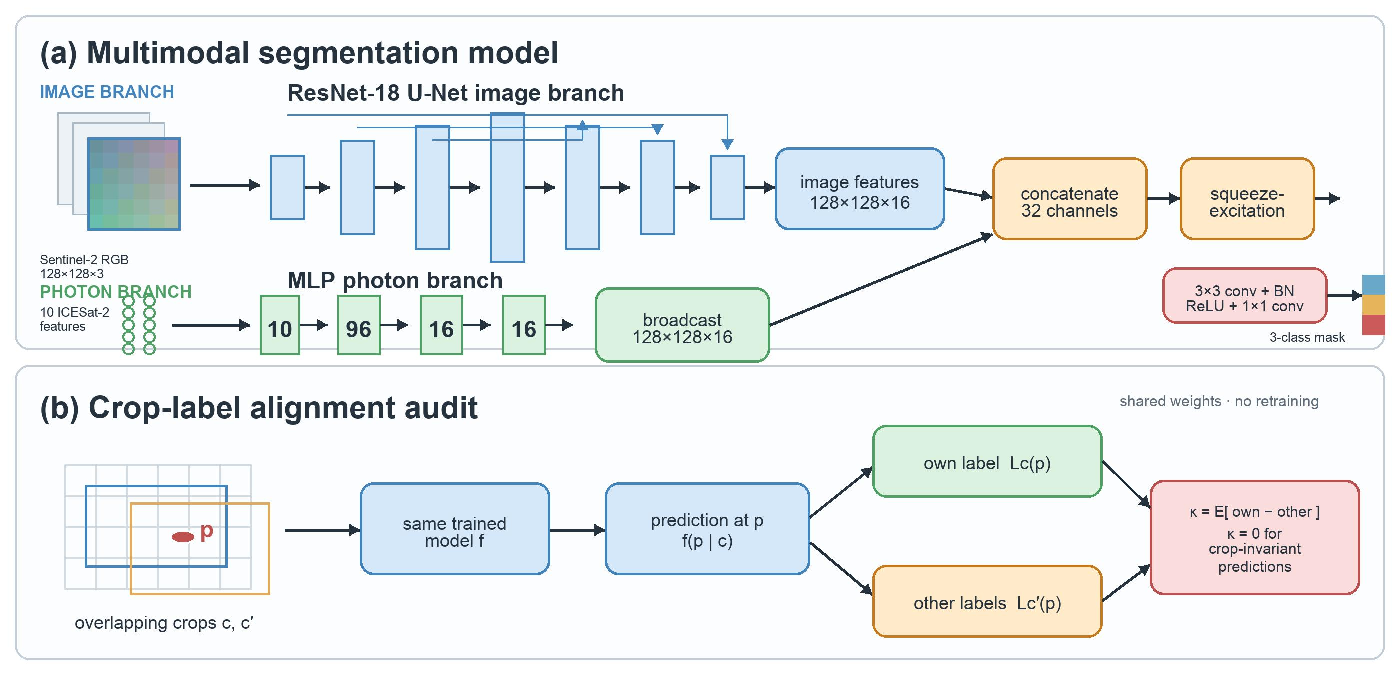
\includegraphics[width=\textwidth]{figures/crop_alignment_architecture.pdf}
\caption{Code-faithful model and audit. An ImageNet-initialized~\cite{deng2009imagenet}
ResNet-18~\cite{he2016resnet} U-Net~\cite{ronneberger2015unet} encodes each image;
an MLP encodes the photon features; and squeeze--excitation~\cite{hu2018senet}
fuses them. The audit sends overlapping crops through shared weights and compares
agreement with the current crop's label against other crops' labels for the same
source pixel.}
\label{fig:architecture}
\end{figure*}

\begin{table}[tb]
\centering
\footnotesize
\setlength{\tabcolsep}{2.2pt}
\begin{tabular}{lccc}
\toprule
 & ice & flood-chip & flood-crop \\
\midrule
input & RGB+10 & VV,VH & VV,VH \\
crop/stride & 128/-- & 512/-- & 128/32 \\
LR & 1e-4 & 3e-4 & 3e-4 \\
loss & focal & CE & CE \\
batch & 128 & 8 & 32 \\
cap/pat. & 12/5;60/15;120/15 & 40/10 & 20/6 \\
held out & acquisition & event & event \\
folds & 17 (16 $\kap$) & 11 & 11 \\
seeds & 42,7,123 & 42,7,123 & 42 \\
\bottomrule
\end{tabular}
\caption{Configuration of the three experimental arms. Crops are square and
sizes are in pixels. CE denotes cross-entropy.}
\label{tab:setup}
\end{table}

The sea-ice benchmark contains 169{,}051 patches over 39 tiles and 17
acquisitions; the flood benchmark has 446 chips over 11 events. The crop sweep
draws 24 crops per chip per epoch and evaluates $\kap$ on all 169 positions of a
$13\times13$ grid. The ten co-registered ICESat-2 photon
features~\cite{neumann2019atlas} form the second model branch in
\cref{fig:architecture}; that branch is held fixed across every arm.

Splits are leave-one-acquisition-out or leave-one-event-out, the unit sharing a
labeller constant. Validation uses 15\% of the remaining units and never the held-out
unit. A tile-disjoint arm also forbids tiles from crossing train and test. The 12-epoch
sea-ice arm uses shorter patience, so it is not a pure cap change. Reported runs used
two RTX A6000 cards capped at 300\,W: sea-ice folds took 41--67 minutes at 60 epochs
and 49--149 at 120; flood crop runs took about four minutes.

\section{The instrument in the wild}
\label{sec:wild}

\subsection{Two labellers, recovered exactly}
\label{sec:recovery}

\paragraph{Sea ice.} The labeller of~\cite{iqrah2023polar}, scaled with cloud and
shadow removal in~\cite{iqrah2024parallel}, applies HSV thresholds to each RGB patch
after background subtraction. The thresholds admit hue 0 to 185 while OpenCV hue
ranges 0 to 179, so hue and saturation constrain nothing and only the value channel
acts. A two-parameter grid search recovers the water constant in 17 of 17 folds.
Otsu and two min-max normalisations are recomputed on each $128 \times 128$ patch,
so a pixel's label depends on the framing of its crop. Regenerating once per scene
makes the labels exactly crop-invariant: crop unanimity is $1.0000$ on all 17 folds
for the repaired scheme against $0.9678$ for the original.

\paragraph{Floods.} Sen1Floods11 ships an expert label and an Otsu label for the
same 446 chips, and unlike the sea-ice case it publishes the constant, so the
recovery can be checked from outside. Recovery from the raw band gives 94.9\% pixel
agreement but sits 1.19\,dB low on all ten events with a published value. A bias of
one sign everywhere is a signature, not noise. Sweeping the smoothing radius,
the bias crosses zero at a $9 \times 9$ focal mean, where 10 of 10 events land within
0.25\,dB at 99.05\% agreement (\cref{fig:recovery}). The constant moves 5.57\,dB
across events, so no global threshold can express it and a model seeing the whole
chip can infer which event it is in and adapt.

\begin{figure}[tb]
\centering
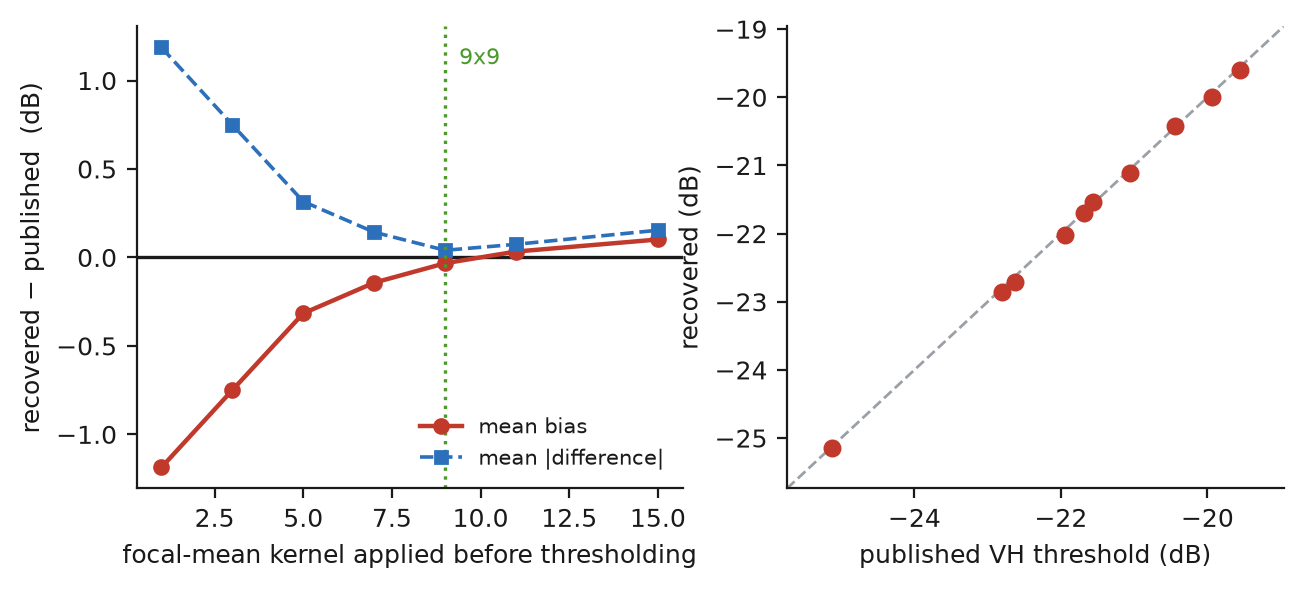
\includegraphics[width=\linewidth]{figures/label_generator_recovery.png}
\caption{Recovering the flood labeller. Left: bias and mean absolute difference
against the published thresholds as the smoothing kernel is swept. Right: recovered
against published threshold, one point per event.}
\label{fig:recovery}
\end{figure}

\subsection{Crop alignment on the sea-ice benchmark}

Sea-ice crops overlap about 33 times, so a source pixel is seen inside many crops,
and under the per-crop scheme those crops can disagree. For the 16 folds with
committed machine-readable results, $\A$ averages 13.58\% of covered pixels. The
model trained on crop-noisy labels reads $\kap=+0.1230$ (sd $0.0361$); the matched
control, trained on repaired labels and evaluated on identical pixels, reads
$+0.0157$. Their paired difference is $\mathbf{+0.1073}$ (sd $0.0333$,
$t=12.88$, positive in 16 of 16 folds, two-sided sign test $p=0.000031$).
\Cref{fig:wild} shows all machine-readable folds. The power formula returns a value
below two, where a paired variance cannot be estimated, so we do not quote a
required sample size.

The released text summary contains a rounded seventeenth row, but the corresponding
per-fold JSON is absent. Including it would change the paired difference to
$+0.1106$. We exclude that row from every headline result rather than silently
mixing machine-readable evidence with an unreconstructable summary.

\begin{figure}[tb]
\centering
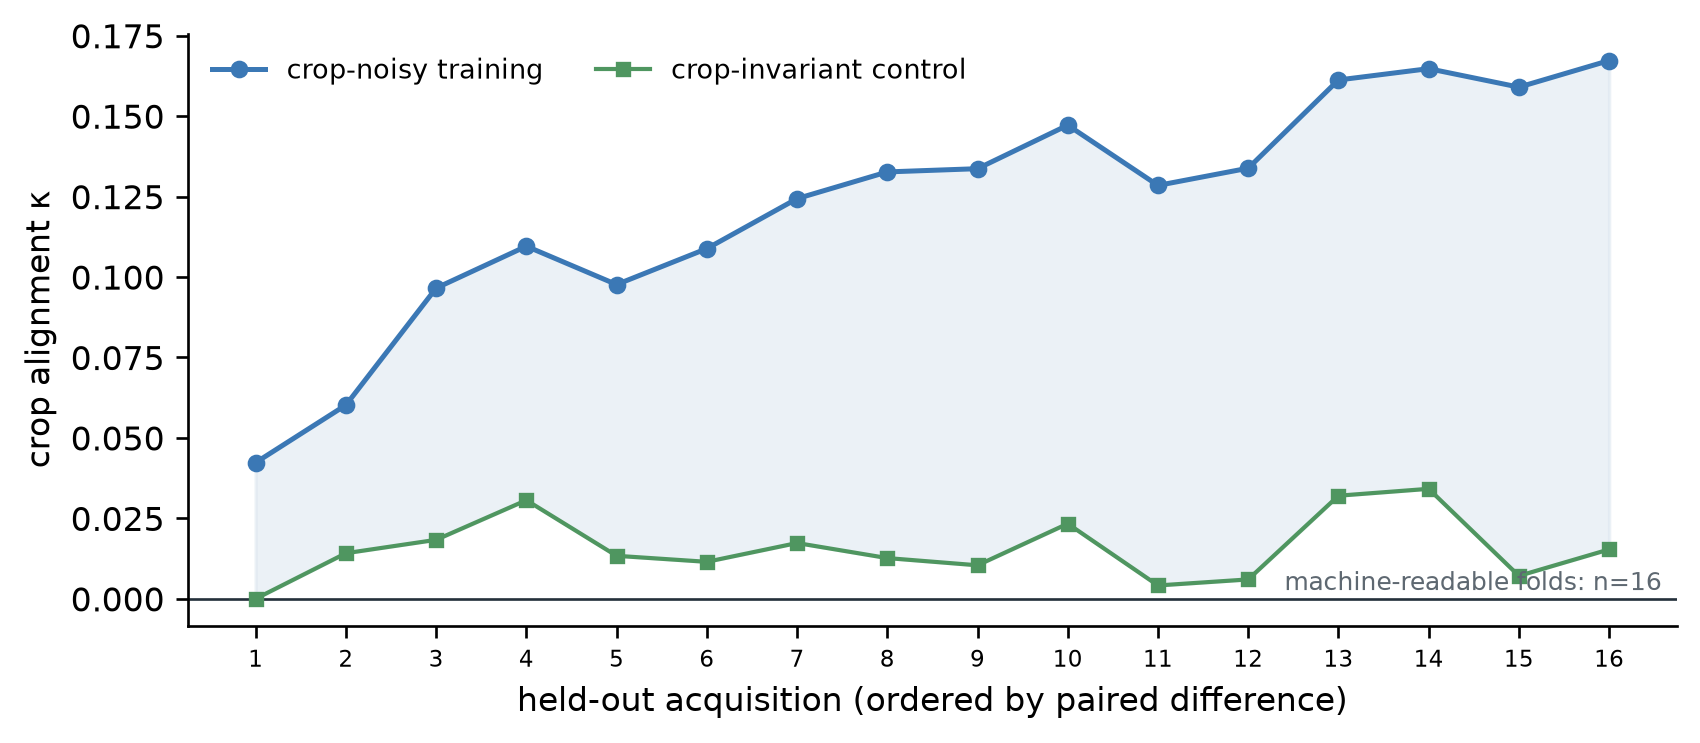
\includegraphics[width=\linewidth]{figures/crop_alignment_results.png}
\caption{Crop alignment for the 16 held-out acquisitions with machine-readable
evidence, each against its matched control. The zero line is the structural null of
\cref{prop:null}, not an estimated baseline.}
\label{fig:wild}
\end{figure}

We do not divide this by the calibrated contrast of \Cref{sec:calib} to express it
as a fraction of a fully closed-loop labeller. The two were measured on different
crop grids, and \Cref{sec:grid} shows a grid change moves the contrast by more than
any such ratio would report.

Two consistency checks follow. On the repaired label set $\A$ is empty, since crop unanimity
of $1.0000$ on all 17 folds means every covering crop agrees. And $\Omega$ is exactly
zero for the two-parameter threshold, because the value channel is a per-pixel
function and the thresholds are per-fold constants.

\subsection{What the closed loop costs against a human}

Sea ice has no reference labels, so it can show that a model learns the labeller but
not what that costs. Sen1Floods11 has both. Training on each label set and scoring
both against the expert labels on the same held-out event gives a transfer collapse
of $-0.0454$ mIoU (sd $0.0470$, $t = -3.21$, negative in 9 of 11 events, two-sided
sign test $p = 0.065$). Model input is Sentinel-1 throughout, since the expert labels
were produced by analysts correcting a Sentinel-2 classification and the reference
arm is open-loop only while the model never reads Sentinel-2.

The mechanism check is harder to explain away. If the collapse comes from learning a
labeller rather than a phenomenon, it must be largest where labeller and human
disagree most, and it is. The correlation between label agreement and collapse is
$+0.719$ with a regression slope at $t = +3.11$. Events where the label sets agree
least collapse by $-0.0571$ against $-0.0314$ where they agree most, a ratio of
$1.8\times$.

\section{What these benchmarks can resolve}
\label{sec:resolution}

Throughout we take the acquisitions needed to detect an effect $d$ at 80\% power
and two-sided $\alpha = 0.05$ as $n = (2.80\,s/d)^2$, with $s$ the paired per-fold
standard deviation, $2.80 = z_{0.975} + z_{0.80}$. Each of our effects carries its
measured paired spread. The normal approximation understates the paired $t$-test
requirement by two to three at these sample sizes, so the values are planning
approximations rather than exact thresholds.

\begin{figure}[tb]
\centering
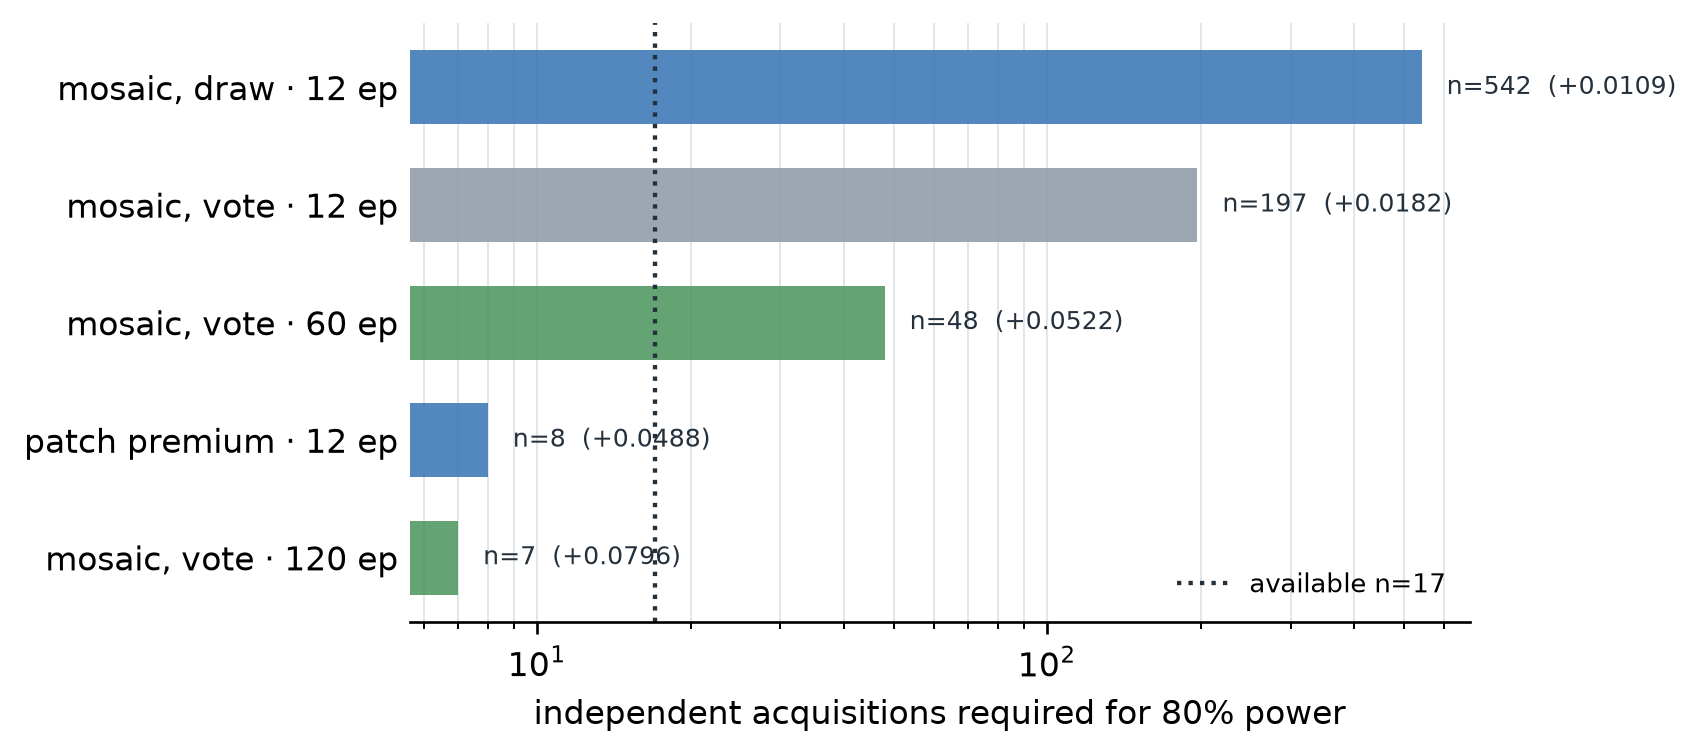
\includegraphics[width=\linewidth]{figures/required_sample_size.png}
\caption{Acquisitions required to detect our artefact-premium estimates at 80\%
power, log axis. The vertical line marks the 17 available acquisitions. Green bars
are longer-budget sensitivity results supported by summary logs rather than
per-run JSON and checkpoints.}
\label{fig:power}
\end{figure}

We define the \emph{artefact premium} as a difference in differences: the mIoU gap
between a U-Net and a context-free threshold baseline on the closed-loop labels,
minus the same gap on the repaired labels, with both arms scored on identical
pixels. It is the share of the network's apparent advantage that survives only
because of how the labeller was implemented. The same power calculation applies to
it.

\begin{table}[tb]
\centering
\small
\setlength{\tabcolsep}{4pt}
\begin{tabular}{lcccc}
\toprule
 & premium & sd & $t$ & required $n$ \\
\midrule
\multicolumn{5}{l}{\emph{scoring convention, at the 12-epoch budget}} \\
patch pixels & $+0.0488$ & $0.0489$ & $4.12$ & 8 \\
mosaic, vote & $+0.0182$ & $0.0910$ & $0.82$ & 197 \\
mosaic, draw & $+0.0109$ & $0.0903$ & $0.50$ & 542 \\
\midrule
\multicolumn{5}{l}{\emph{training budget, under mosaic-vote scoring}} \\
12 epochs & $+0.0182$ & $0.0910$ & $0.82$ & 197 \\
60 epochs & $+0.0522$ & $0.1290$ & $1.67$ & 48 \\
120 epochs & $\mathbf{+0.0796}$ & $\mathbf{0.0747}$ & $\mathbf{4.39}$ & $\mathbf{7}$ \\
\bottomrule
\end{tabular}
\caption{The artefact premium under three scoring conventions and, below, at three
training budgets on the same 17 folds, with the sample size each would need at 80\%
power. Budget aggregates come from the committed run log; per-run JSON and
checkpoints for the 120-epoch arm are not in the release.}
\label{tab:premium}
\end{table}

Patch-pixel scoring needs 8 acquisitions and therefore resolves, but mosaic scoring,
which counts each source pixel once, needs 197 and does not. Applying that convention
to our own result shrinks the premium $2.7\times$ and removes significance. The draw
convention is still more conservative. Estimating rather than fixing the threshold
coefficient gives $\hat\beta=0.711$ (se $0.175$); under it, the patch-scored premium
falls to $t=1.81$.

\paragraph{Training budget.} The committed log reports that the mosaic premium rises
from $+0.0182$ to $+0.0796$ between 12 and 120 epochs, with the change positive in all
17 folds ($t=3.98$); required $n$ falls from 197 to 7. The runner records a
pre-result stopping criterion: 21 of 34 runs reached the 60-epoch cap without early
stopping, compared with 2 of 34 at 120. The 120-epoch result survives every
leave-one-out analysis (minimum $t=4.02$) and four missing-class conventions. These
are useful sensitivity checks, but they remain log-level evidence because the
release lacks their per-run JSON and checkpoints. We therefore do not use them in
the abstract or conclusion.

\paragraph{Multiplicity.} This paper reports many tests, and the results it rests on
are not close to the boundary. Crop alignment at $t = 12.88$ and the dose-response at
$t = 29.84$ would not change interpretation under a Bonferroni factor of 100. The cost
at $t = -4.27$ is $p = 0.0016$ on 10 degrees of freedom, so it tolerates a factor of
about 30 and not 100, which we state because it is the weakest of the three. One
secondary result sits where multiplicity matters and should be read as suggestive: the
transfer collapse sign test at $p = 0.065$. We apply no blanket correction, because a
structural null and an estimated contrast are not the same kind of object.

\section{Recommendations}
\label{sec:recs}

Generate labels once per scene, preserve nodata as an ignore class, split by
acquisition with a receptive-field buffer, and score each source pixel once by
mosaicking. Report a context-free baseline, $\kap$ and its matched control on a stated
crop grid, and the required number of independent units. An empty artefact set means
that $\kap$ cannot be estimated; the implementation reports this state explicitly,
and it must not be read as evidence that the labels are shortcut-free.

\section{Limitations}
\label{sec:limits}

\paragraph{Diagnostic scope.} $\kap$ requires overlapping crops whose labels
disagree. It cannot test a crop-invariant automatic labeller, a scene-level
pseudo-label shortcut, or any shortcut unrelated to crop geometry. An empty
artefact set is therefore outside the estimand, not a successful negative result.

\paragraph{Identification.} Nonzero $\kap$ certifies crop-dependent predictions on
the artefact set. Even a positive treatment--control contrast does not uniquely
prove that the network copied the labelling algorithm: the matched control estimates
an architecture and optimisation floor, but label difficulty and training dynamics
can still differ between arms. The result is a targeted diagnostic, not a causal
mediation analysis.

\paragraph{Scale and external validity.} We study two remote-sensing domains, two
sensors, and two labelling families. Sea ice contributes 17 acquisitions and floods
eleven events. The flood artefact is constructed and is absent from Sen1Floods11 as
published; sea ice has no human reference labels. Neither setting establishes how
often the failure occurs elsewhere.

\paragraph{Estimand dependence.} $\kap$ is relative to the chosen crop size, stride,
and weighting, so its magnitude does not travel between papers. It also does not
directly quantify score inflation: our unfitted prediction $P(\A)\kap$ gets the sign
right on 14 of 17 folds but misses the magnitude by a factor of 1.6--1.9 and has
fold-level rank correlation $+0.216$.

\paragraph{Evidence boundary.} The machine-readable sea-ice summary contains 16
paired fold values, while a rounded text report contains an unmatched seventeenth.
The flood dial and accuracy-cost event rows and the 60/120-epoch aggregates are also
committed as summary logs. Raw predictions, checkpoints, and some per-run JSON are
absent. The release therefore verifies the arithmetic of the supported aggregates;
it does not reproduce training or regenerate every result end to end. We exclude the
unmatched fold from the main result and keep longer-budget results as sensitivity
evidence. The supplement inventories these tiers and the claims withdrawn from
earlier drafts.

\section{Conclusion}

Closed-loop labelling is usually discussed as a kind of noise. It is the opposite of
noise, because a model can learn it, and that is why it inflates measured performance
rather than depressing it. We gave a test whose null follows from the definition
rather than from a control arm, verified it against a case with a known answer,
calibrated it on a labeller we could turn up and down, and showed that what it detects
costs accuracy against human annotation. On the benchmark where the artefact occurred
naturally the paired contrast is $+0.1073$ across all 16 folds with machine-readable
evidence. At the initial mosaic-scored budget, however, the aggregate artefact
premium itself is unresolved (required $n=197$ versus 17 available acquisitions),
and the stronger longer-budget result is summary-log evidence only. Crop alignment
makes one specific shortcut measurable; the provenance audit defines which claims
the current release can support.


\paragraph{Code and data.}
\iftoggle{wacvfinal}{The reproducibility package is available at
\url{https://github.com/kacytran1122/crop-alignment}.}{Code and auditable
artifacts are included in the anonymous supplementary submission. The public URL
is withheld during double-blind review and is enabled in the camera-ready source.}

{
    \small
    \bibliographystyle{ieeenat_fullname}
    \bibliography{references}
}

\end{document}
